\documentclass[11pt]{article}
\usepackage[margin=1in]{geometry}
\usepackage{amsmath,amssymb,mathtools}
\usepackage{graphicx}
\usepackage{booktabs}
\usepackage{enumitem}

\newcommand{\E}{\mathbb{E}}
\newcommand{\R}{\mathbb{R}}
\newcommand{\N}{\mathcal{N}}
\newcommand{\KL}{D_{\mathrm{KL}}}
\newcommand{\vx}{\mathbf{x}}
\newcommand{\veps}{\boldsymbol{\epsilon}}
\newcommand{\vzero}{\mathbf{0}}
\newcommand{\Id}{I}

\title{EE/CS 148B HW 4 Derivations}
\author{}
\date{}

\begin{document}
\maketitle

\subsection*{Problem 1.2: Variational Bound}
The likelihood $p_\theta(x_0)=\int p_\theta(x_{0:T})\,dx_{1:T}$ is generally intractable because it requires integrating over all latent diffusion states.  We therefore optimize a variational upper bound on the negative log likelihood; equivalently, we maximize the usual evidence lower bound.

For any forward process $q(x_{1:T}\mid x_0)$ whose support contains the support of $p_\theta(x_{0:T})$,
\begin{align*}
-\log p_\theta(x_0)
&= -\log \int p_\theta(x_{0:T})\,dx_{1:T} \\
&= -\log \int q(x_{1:T}\mid x_0)
       \frac{p_\theta(x_{0:T})}{q(x_{1:T}\mid x_0)}\,dx_{1:T} \\
&\leq \E_q\left[-\log
       \frac{p_\theta(x_{0:T})}{q(x_{1:T}\mid x_0)}\right],
\end{align*}
where the inequality is Jensen's inequality applied to the convex function $-\log(\cdot)$.  Taking expectation over $q(x_0)$ gives
\begin{align*}
\E[-\log p_\theta(x_0)]
&\leq
\E_q\left[-\log
       \frac{p_\theta(x_{0:T})}{q(x_{1:T}\mid x_0)}\right].
\end{align*}
Using
\[
p_\theta(x_{0:T})=p(x_T)\prod_{t=1}^T p_\theta(x_{t-1}\mid x_t),
\qquad
q(x_{1:T}\mid x_0)=\prod_{t=1}^T q(x_t\mid x_{t-1}),
\]
the bound becomes
\begin{align*}
\E[-\log p_\theta(x_0)]
&\leq
\E_q\left[
-\log p(x_T)
-\sum_{t\geq 1}
\log \frac{p_\theta(x_{t-1}\mid x_t)}{q(x_t\mid x_{t-1})}
\right]
 =: L.
\end{align*}

\subsection*{Problem 1.3: Tractable Loss Function}
Equation (18) follows by substituting the Markov factorizations of the reverse and forward processes into Eq. (17):
\begin{align*}
L
&=\E_q\left[-\log \frac{p_\theta(x_{0:T})}{q(x_{1:T}\mid x_0)}\right] \\
&=\E_q\left[-\log p(x_T)
-\sum_{t\geq 1}\log p_\theta(x_{t-1}\mid x_t)
+\sum_{t\geq 1}\log q(x_t\mid x_{t-1})\right] \\
&=\E_q\left[-\log p(x_T)
-\sum_{t\geq 1}\log
\frac{p_\theta(x_{t-1}\mid x_t)}{q(x_t\mid x_{t-1})}\right].
\end{align*}

Equation (20) uses Bayes' rule and the Markov property of the forward chain:
\[
q(x_{t-1}\mid x_t,x_0)
=\frac{q(x_t\mid x_{t-1},x_0)q(x_{t-1}\mid x_0)}{q(x_t\mid x_0)}
=\frac{q(x_t\mid x_{t-1})q(x_{t-1}\mid x_0)}{q(x_t\mid x_0)}.
\]
Thus
\[
q(x_t\mid x_{t-1})
=q(x_{t-1}\mid x_t,x_0)\frac{q(x_t\mid x_0)}{q(x_{t-1}\mid x_0)},
\]
which is substituted into the denominator of Eq. (19).

Equation (21) follows from telescoping the marginal terms:
\begin{align*}
&-\sum_{t>1}\log \frac{q(x_{t-1}\mid x_0)}{q(x_t\mid x_0)}
+\log q(x_1\mid x_0) \\
&\qquad
=-\log\frac{q(x_1\mid x_0)}{q(x_T\mid x_0)}
+\log q(x_1\mid x_0)
=\log q(x_T\mid x_0).
\end{align*}
This combines with $-\log p(x_T)$ to give $-\log \frac{p(x_T)}{q(x_T\mid x_0)}$.

Equation (22) is the definition of KL divergence applied inside the expectation:
\begin{align*}
\E_q\left[-\log \frac{p(x_T)}{q(x_T\mid x_0)}\right]
&= \KL(q(x_T\mid x_0)\,\|\,p(x_T)),\\
\E_q\left[-\log
\frac{p_\theta(x_{t-1}\mid x_t)}
{q(x_{t-1}\mid x_t,x_0)}\right]
&= \KL(q(x_{t-1}\mid x_t,x_0)\,\|\,p_\theta(x_{t-1}\mid x_t)).
\end{align*}
The decoder term remains $-\log p_\theta(x_0\mid x_1)$.

\subsection*{Problem 1.4: Markov Process -- Equation (4)}
The forward transition can be reparameterized as
\[
x_t=\sqrt{\alpha_t}x_{t-1}+\sqrt{\beta_t}z_t,\qquad z_t\sim\N(0,\Id),
\]
where $\alpha_t=1-\beta_t$.  If
\[
x_{t-1}=\sqrt{\bar\alpha_{t-1}}x_0+\sqrt{1-\bar\alpha_{t-1}}\,\epsilon_{t-1},
\]
then
\begin{align*}
x_t
&=\sqrt{\alpha_t\bar\alpha_{t-1}}x_0
+\sqrt{\alpha_t(1-\bar\alpha_{t-1})}\,\epsilon_{t-1}
+\sqrt{\beta_t}z_t.
\end{align*}
The last two terms are independent Gaussians with total covariance
\[
\alpha_t(1-\bar\alpha_{t-1})\Id+\beta_t\Id
=(1-\alpha_t\bar\alpha_{t-1})\Id
=(1-\bar\alpha_t)\Id.
\]
Therefore
\[
q(x_t\mid x_0)=\N\left(x_t;\sqrt{\bar\alpha_t}x_0,(1-\bar\alpha_t)\Id\right).
\]

\subsection*{Problem 1.5: Markov Process -- Equations (6) and (7)}
Conditioned on $x_0$,
\[
x_{t-1}\sim \N(\sqrt{\bar\alpha_{t-1}}x_0,(1-\bar\alpha_{t-1})\Id),
\]
and
\[
x_t=\sqrt{\alpha_t}x_{t-1}+\sqrt{\beta_t}z_t.
\]
Hence $(x_{t-1},x_t)\mid x_0$ is jointly Gaussian with
\begin{align*}
\mu_{t-1}&=\sqrt{\bar\alpha_{t-1}}x_0,&
\mu_t&=\sqrt{\bar\alpha_t}x_0,\\
\Sigma_{t-1,t-1}&=(1-\bar\alpha_{t-1})\Id,&
\Sigma_{t,t}&=(1-\bar\alpha_t)\Id,\\
\Sigma_{t-1,t}&=\sqrt{\alpha_t}(1-\bar\alpha_{t-1})\Id.
\end{align*}
The Gaussian conditioning formula gives
\begin{align*}
q(x_{t-1}\mid x_t,x_0)
&=\N(x_{t-1};\tilde\mu_t(x_t,x_0),\tilde\beta_t\Id),\\
\tilde\mu_t(x_t,x_0)
&=\mu_{t-1}
\Sigma_{t-1,t}\Sigma_{t,t}^{-1}(x_t-\mu_t)\\
&=\frac{\sqrt{\bar\alpha_{t-1}}\beta_t}{1-\bar\alpha_t}x_0
+\frac{\sqrt{\alpha_t}(1-\bar\alpha_{t-1})}{1-\bar\alpha_t}x_t,
\end{align*}
and
\begin{align*}
\tilde\beta_t\Id
&=\Sigma_{t-1,t-1}-\Sigma_{t-1,t}\Sigma_{t,t}^{-1}\Sigma_{t,t-1}\\
&=\left((1-\bar\alpha_{t-1})
-\frac{\alpha_t(1-\bar\alpha_{t-1})^2}{1-\bar\alpha_t}\right)\Id\\
&=\frac{1-\bar\alpha_{t-1}}{1-\bar\alpha_t}\beta_t\Id.
\end{align*}

\subsection*{Problem 1.6: KL Divergence and Equation (8)}
For $p=q(x_{t-1}\mid x_t,x_0)=\N(\tilde\mu_t,\tilde\beta_t\Id)$ and
$q=p_\theta(x_{t-1}\mid x_t)=\N(\mu_\theta,\beta_t\Id)$, the Gaussian KL formula gives
\[
\KL(p\,\|\,q)
=\frac12\left[
\log\frac{|\beta_t\Id|}{|\tilde\beta_t\Id|}
-d+\mathrm{tr}\big((\beta_t\Id)^{-1}\tilde\beta_t\Id\big)
+(\mu_\theta-\tilde\mu_t)^\top(\beta_t\Id)^{-1}(\mu_\theta-\tilde\mu_t)
\right].
\]
The log determinant, $-d$, and trace terms do not depend on $\theta$.  Therefore, after absorbing them into a constant $C$,
\[
L_{t-1}-C
=\E_q\left[\frac{1}{2\beta_t}
\|\tilde\mu_t(x_t,x_0)-\mu_\theta(x_t,t)\|^2\right].
\]

\subsection*{Problem 1.7: Parameterization and Equation (12)}
Let
\[
x_t(x_0,\epsilon)=\sqrt{\bar\alpha_t}x_0+\sqrt{1-\bar\alpha_t}\epsilon.
\]
Equation (10) contains
\[
\frac{1}{\sqrt{\alpha_t}}
\left(x_t-\frac{\beta_t}{\sqrt{1-\bar\alpha_t}}\epsilon\right)
-\mu_\theta(x_t,t).
\]
Using Eq. (11),
\[
\mu_\theta(x_t,t)
=\frac{1}{\sqrt{\alpha_t}}
\left(x_t-\frac{\beta_t}{\sqrt{1-\bar\alpha_t}}\epsilon_\theta(x_t,t)\right).
\]
Subtracting gives
\[
\frac{\beta_t}{\sqrt{\alpha_t}\sqrt{1-\bar\alpha_t}}
\left(\epsilon_\theta(x_t,t)-\epsilon\right).
\]
Thus
\[
L_{t-1}-C
=\E_{x_0,\epsilon}\left[
\frac{\beta_t^2}{2\sigma_t^2\alpha_t(1-\bar\alpha_t)}
\left\|
\epsilon-\epsilon_\theta\left(\sqrt{\bar\alpha_t}x_0+\sqrt{1-\bar\alpha_t}\epsilon,t\right)
\right\|^2
\right].
\]

\subsection*{Problem 1.8: Coefficient Plot}
With $\sigma_t^2=\beta_t$, the coefficient is
\[
\frac{\beta_t^2}{2\sigma_t^2\alpha_t(1-\bar\alpha_t)}
=
\frac{\beta_t}{2\alpha_t(1-\bar\alpha_t)}.
\]
The plot below uses the DDPM linear schedule $T=1000$, $\beta_1=10^{-4}$, and $\beta_T=0.02$.
\begin{center}
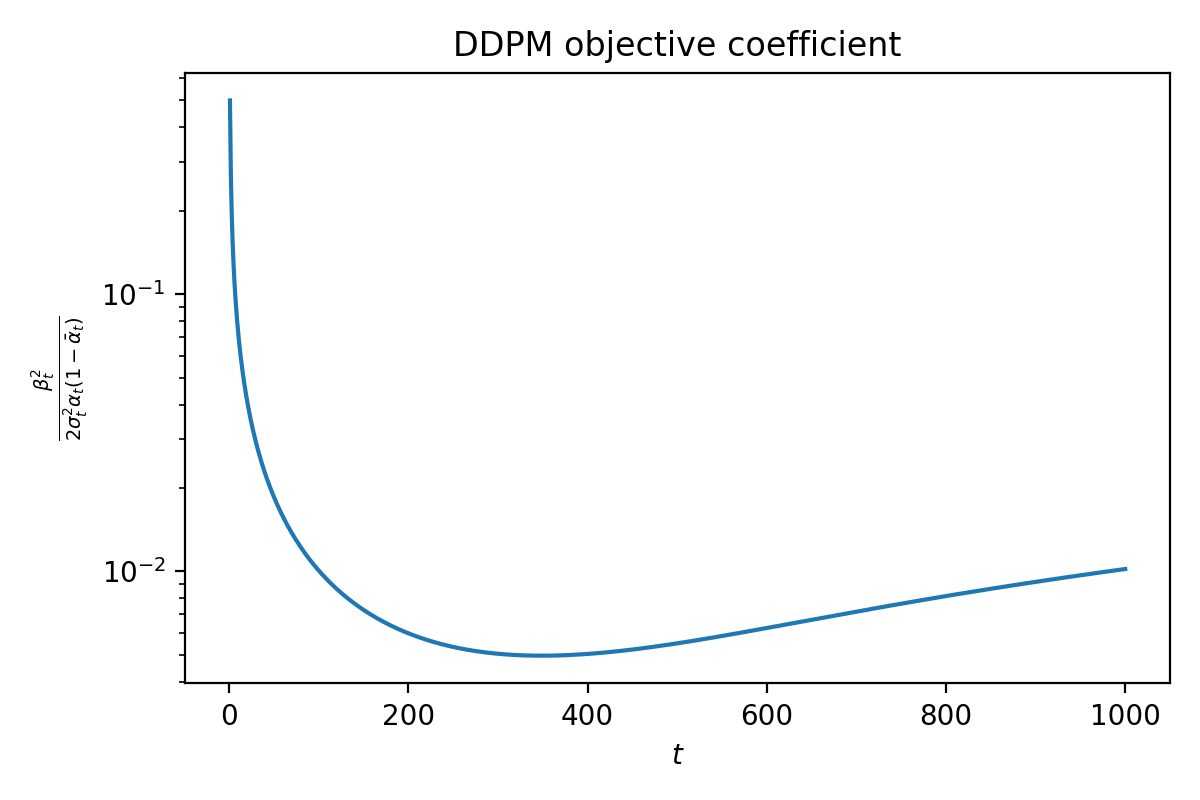
\includegraphics[width=0.7\linewidth]{figures/problem_1_8_coefficient.png}
\end{center}

\subsection*{Problem 2.2: Explicit Score Matching}
The explicit score matching objective requires the true data score $\nabla_x\log p(x)$.  In image generation we usually only have samples from the data distribution, not an evaluable density $p(x)$ or its gradient.  Even if an unnormalized density were available, its score can be analytically or computationally intractable in high dimensions.

\subsection*{Problem 2.3: Implicit Score Matching}
Expanding the explicit score matching objective,
\begin{align*}
J_{\mathrm{ESM}}(\theta)
&=\E_p\left[\frac12\|s_\theta(x)\|^2
-s_\theta(x)^\top\nabla_x\log p(x)
+\frac12\|\nabla_x\log p(x)\|^2\right].
\end{align*}
The final term is independent of $\theta$.  For the cross term,
\begin{align*}
\E_p[s_\theta(x)^\top\nabla_x\log p(x)]
&=\int s_\theta(x)^\top\nabla_x p(x)\,dx\\
&=\sum_i \int s_{\theta,i}(x)\,\partial_i p(x)\,dx\\
&=\sum_i \left([s_{\theta,i}(x)p(x)]_{\partial\Omega}
-\int p(x)\partial_i s_{\theta,i}(x)\,dx\right).
\end{align*}
Because $p(x)$ vanishes at infinity, the boundary term is zero.  Therefore
\[
\E_p[s_\theta(x)^\top\nabla_x\log p(x)]
=-\E_p[\mathrm{tr}(\nabla_x s_\theta(x))].
\]
Substitution gives
\[
J_{\mathrm{ESM}}(\theta)
=\E_p\left[
\mathrm{tr}(\nabla_xs_\theta(x))+\frac12\|s_\theta(x)\|^2
\right]+\mathrm{const.}
=J_{\mathrm{ISM}}(\theta)+\mathrm{const.}
\]

\subsection*{Problem 2.4: Limitation of ISM}
Implicit score matching avoids the unknown data score, but it requires the divergence $\mathrm{tr}(\nabla_x s_\theta(x))$.  For neural networks on high-dimensional images, computing this trace exactly is expensive and often requires higher-order automatic differentiation, making the objective less attractive in practice.

\subsection*{Problem 2.5: Tweedie's Formula}
Let $\tilde x=x+\sigma\epsilon$ with $\epsilon\sim\N(0,\Id)$.  The noisy marginal density is
\[
p_\sigma(\tilde x)=\int p(x)\,\N(\tilde x;x,\sigma^2\Id)\,dx.
\]
Taking a gradient with respect to $\tilde x$,
\begin{align*}
\nabla_{\tilde x}p_\sigma(\tilde x)
&=\int p(x)\nabla_{\tilde x}\N(\tilde x;x,\sigma^2\Id)\,dx\\
&=\int p(x)\N(\tilde x;x,\sigma^2\Id)
\frac{x-\tilde x}{\sigma^2}\,dx\\
&=p_\sigma(\tilde x)\,
\E\left[\frac{x-\tilde x}{\sigma^2}\mid \tilde x\right].
\end{align*}
Dividing by $p_\sigma(\tilde x)$ gives
\[
\nabla_{\tilde x}\log p_\sigma(\tilde x)
=\frac{\E[x\mid \tilde x]-\tilde x}{\sigma^2},
\]
so
\[
\E[x\mid \tilde x]=\tilde x+\sigma^2\nabla_{\tilde x}\log p_\sigma(\tilde x).
\]

\subsection*{Problem 2.6: DSM Objective from Tweedie's Formula}
Tweedie's formula suggests training a denoiser
\[
D_\theta(\tilde x)=\tilde x+\sigma^2s_\theta(\tilde x)
\]
by minimizing $\E\left[\frac12\|D_\theta(\tilde x)-x\|^2\right]$.  This is equivalent, up to the positive factor $\sigma^4$, to minimizing
\[
\E_{p(x)}\E_{p(\tilde x\mid x)}
\left[
\frac12\left\|s_\theta(\tilde x)-\frac{x-\tilde x}{\sigma^2}\right\|^2
\right].
\]
Since
\[
\nabla_{\tilde x}\log p(\tilde x\mid x)
=\nabla_{\tilde x}\log \N(\tilde x;x,\sigma^2\Id)
=\frac{x-\tilde x}{\sigma^2},
\]
this is exactly $J_{\mathrm{DSM}}(\theta;\sigma)$.

Equivalently, let
\[
u(x,\tilde x)=\nabla_{\tilde x}\log p(\tilde x\mid x).
\]
By the law of total expectation,
\[
\E[u(x,\tilde x)\mid \tilde x]
=\nabla_{\tilde x}\log p_\sigma(\tilde x).
\]
Then
\begin{align*}
\E\|s_\theta(\tilde x)-u\|^2
&=\E\|s_\theta(\tilde x)-\E[u\mid \tilde x]\|^2
+\E\|u-\E[u\mid \tilde x]\|^2,
\end{align*}
where the second term is independent of $\theta$.  Hence the DSM objective has the same optimizer as score matching against the noisy marginal score.

\subsection*{Problem 2.7: DSM vs. DDPM}
At DDPM time $t$,
\[
x_t=\sqrt{\bar\alpha_t}x_0+\sqrt{1-\bar\alpha_t}\epsilon
=\sqrt{\bar\alpha_t}x_0+\sigma\epsilon,
\qquad \sigma=\sqrt{1-\bar\alpha_t}.
\]
The conditional score of the perturbation kernel is
\[
\nabla_{x_t}\log q(x_t\mid x_0)
=-\frac{x_t-\sqrt{\bar\alpha_t}x_0}{1-\bar\alpha_t}
=-\frac{\epsilon}{\sigma}.
\]
Thus the DSM target is $-\epsilon/\sigma$, while the simplified DDPM objective predicts $\epsilon$.  If $\epsilon_\theta^*$ is the DDPM optimizer at time $t$, then the DSM optimizer is
\[
s_\theta^*(x_t,t)=c(\sigma)\epsilon_\theta^*(x_t,t),
\qquad
c(\sigma)=-\frac{1}{\sigma}.
\]

\subsection*{Problem 2.8: Langevin Dynamics Sampling}
After training $s_\theta(x)\approx \nabla_x\log p_\sigma(x)$, initialize $x_0$ from a broad distribution such as a Gaussian.  For small step size $\eta$, iterate
\[
x_{k+1}=x_k+\eta s_\theta(x_k)+\sqrt{2\eta}\,z_k,
\qquad z_k\sim\N(0,\Id),
\]
for many steps.  If $\sigma$ is small, the stationary distribution $p_\sigma$ is close to $p$, so the final $x_K$ is an approximate sample from the target distribution.  In practice, one often anneals from large $\sigma$ to small $\sigma$ to improve mixing.

\subsection*{Problem 3.2: VP-SDE Approximations}
The DDPM discretization can be written with $\Delta t=1/N$ as
\[
x(t+\Delta t)=\sqrt{1-\beta(t+\Delta t)\Delta t}\,x(t)
+\sqrt{\beta(t+\Delta t)\Delta t}\,z(t).
\]
For $\Delta t\ll 1$, Taylor expansion gives
\[
\sqrt{1-\beta(t+\Delta t)\Delta t}
=1-\frac12\beta(t+\Delta t)\Delta t+O(\Delta t^2).
\]
Since $\beta$ is continuous, $\beta(t+\Delta t)=\beta(t)+O(\Delta t)$, and the drift term may be written with $\beta(t)$ up to higher-order error.  Finally, $\sqrt{\Delta t}\,z(t)$ is the Brownian increment $dB_t$ over a time interval of length $\Delta t$.  Taking $\Delta t\to 0$ yields
\[
dx=-\frac12\beta(t)x\,dt+\sqrt{\beta(t)}\,dB_t.
\]

\subsection*{Problem 3.3: Reverse VP-SDE}
For the VP-SDE,
\[
f(x,t)=-\frac12\beta(t)x,\qquad g(t)=\sqrt{\beta(t)}.
\]
The general reverse-time SDE is
\[
dx=\left[f(x,t)-g(t)^2\nabla_x\log p_t(x)\right]dt+g(t)d\bar B_t,
\]
where $dt<0$.  Substituting the VP coefficients gives
\[
dx=\left[-\frac12\beta(t)x-\beta(t)\nabla_x\log p_t(x)\right]dt
+\sqrt{\beta(t)}\,d\bar B_t.
\]

\subsection*{Problem 3.4: Reverse VP-SDE Discretization}
The forward VP discretization is
\[
x_{i+1}=\sqrt{1-\beta_{i+1}}\,x_i+\sqrt{\beta_{i+1}}\,z_i,
\qquad z_i\sim\N(0,\Id),
\]
where $\beta_{i+1}=\bar\beta_{i+1}\Delta t$.  Write this as
\[
x_{i+1}=x_i+f_{i+1}(x_i)+G_{i+1}z_i,
\]
with
\[
f_{i+1}(x)=\left(\sqrt{1-\beta_{i+1}}-1\right)x,
\qquad
G_{i+1}=\sqrt{\beta_{i+1}}\Id.
\]
The reverse-diffusion discretization of the reverse SDE is
\[
x_i=x_{i+1}-f_{i+1}(x_{i+1})
+G_{i+1}G_{i+1}^{\top}s_\theta(x_{i+1},i+1)
+G_{i+1}z_{i+1}.
\]
Substituting $f_{i+1}$ and $G_{i+1}$,
\[
x_i=(2-\sqrt{1-\beta_{i+1}})x_{i+1}
+\beta_{i+1}s_\theta(x_{i+1},i+1)
+\sqrt{\beta_{i+1}}z_{i+1}.
\]
The DDPM ancestral form is
\[
x_i=
\frac{1}{\sqrt{1-\beta_{i+1}}}
\left(x_{i+1}+\beta_{i+1}s_\theta(x_{i+1},i+1)\right)
+\sqrt{\beta_{i+1}}z_{i+1}.
\]
As $\beta_{i+1}\to 0$,
\[
\frac{1}{\sqrt{1-\beta_{i+1}}}=1+\frac12\beta_{i+1}+O(\beta_{i+1}^2),
\qquad
2-\sqrt{1-\beta_{i+1}}=1+\frac12\beta_{i+1}+O(\beta_{i+1}^2).
\]
The extra factor multiplying $\beta_{i+1}s_\theta$ contributes only $O(\beta_{i+1}^2)$, so the two updates agree in the small-step limit.

\subsection*{Problem 3.5: Connecting SDE and DDPM}
The SDE update uses the score term $\beta_t s_\theta(x_t,t)$, while DDPM Algorithm 2 uses
\[
-\frac{\beta_t}{\sqrt{1-\bar\alpha_t}}\epsilon_\theta(x_t,t).
\]
From Problem 2.7,
\[
s_\theta(x_t,t)\approx -\frac{1}{\sqrt{1-\bar\alpha_t}}\epsilon_\theta(x_t,t).
\]
Therefore
\[
\beta_t s_\theta(x_t,t)
\approx
-\frac{\beta_t}{\sqrt{1-\bar\alpha_t}}\epsilon_\theta(x_t,t),
\]
which explains the apparent coefficient difference.

\subsection*{Problem 3.6: Reverse SDE vs. Langevin Dynamics}
Langevin dynamics samples from one target density using only the score of that density.  The reverse SDE uses a whole time-indexed family of scores $\nabla_x\log p_t(x)$ together with the forward drift and diffusion schedule, so it knows how probability mass moves from data to noise across time.

This extra information appears in the continuous score-matching objective because Eq. (7) trains $s_\theta(x,t)$ over all $t$ and matches the perturbation kernel score at each noise level.  It appears in DDPM because Eq. (14) samples a time $t$ and trains the network to denoise at many noise levels, not just at the final data distribution.

\subsection*{Problem 3.7: Conditional Diffusion and Classifier Guidance}
Bayes' rule gives
\[
\log p_t(x\mid y)=\log p_t(x)+\log p_t(y\mid x)-\log p_t(y).
\]
Since $\log p_t(y)$ is constant with respect to $x$,
\[
\nabla_x\log p_t(x\mid y)
=\nabla_x\log p_t(x)+\nabla_x\log p_t(y\mid x).
\]
Classifier guidance estimates the first term with an unconditional score model and the second term with a classifier gradient.  Adding the classifier gradient to the reverse SDE pushes samples toward images likely to have condition $y$ while the unconditional score keeps them on the data manifold.

\subsection*{Problem 4.1: Optimal Velocity Field}
For fixed $t$ and $x$, define $Y=X_1-X_0$.  The rectified flow loss can be minimized pointwise:
\[
\E[\|Y-v(X_t,t)\|^2]
=\E\left[\E[\|Y-v(x,t)\|^2\mid X_t=x]\right].
\]
For each $x,t$, differentiate the inner objective with respect to $v$:
\[
\nabla_v \E[\|Y-v\|^2\mid X_t=x]
=2\left(v-\E[Y\mid X_t=x]\right).
\]
Setting this derivative to zero gives the unique $L^2$ minimizer
\[
v^*(x,t)=\E[X_1-X_0\mid X_t=x].
\]

\subsection*{Problem 4.2: Connection to Score Matching}
Because
\[
X_t=(1-t)X_0+tX_1,
\]
we have, for $t>0$,
\[
X_1-X_0=\frac{X_t-X_0}{t}.
\]
Taking conditional expectation,
\[
v^*(x,t)=\frac{x-\E[X_0\mid X_t=x]}{t}.
\]
Now assume $X_0\sim\N(0,\Id)$.  Since
\[
X_t=tX_1+(1-t)X_0,
\]
the marginal $p_t$ is the data variable $tX_1$ corrupted by Gaussian noise with standard deviation $1-t$.  Its score satisfies
\[
\nabla_x\log p_t(x)
=-\frac{1}{1-t}\E[X_0\mid X_t=x],
\]
so
\[
\E[X_0\mid X_t=x]=-(1-t)\nabla_x\log p_t(x).
\]
Thus
\[
v^*(x,t)=\frac{x+(1-t)\nabla_x\log p_t(x)}{t}.
\]
This shows that the rectified-flow velocity can be expressed through the score of the interpolated marginal distribution.  Rectified flow and score-based diffusion therefore learn closely related conditional expectations, but rectified flow packages the information as a deterministic transport velocity rather than as the reverse drift of a stochastic noising process.

\subsection*{Problem 4.3: Straightness and Reflow}
\begin{enumerate}[label=(\arabic*)]
\item $S=1$ means the integrated velocity exactly equals the endpoint displacement, so the learned path is geometrically straight and one Euler step can recover the endpoint.  $S=0$ means the squared deviation from the endpoint displacement is as large as the displacement energy itself, so the flow has no useful straight-line structure under this metric.
\item Reflow creates new pairs by transporting each sampled noise point through the learned ODE, so the new endpoint is paired with the exact source that generated it.  This removes much of the crossing and mismatch caused by independent noise-data pairing, making the conditional displacement field closer to a constant along each trajectory.
\item One round of reflow costs an additional large sampling pass to create the new paired dataset plus another training run.  Since each round is expensive and improvements usually saturate, practical implementations limit the number of reflow rounds.
\end{enumerate}

\subsection*{Problem 4.4: Rectified Flow vs. DDPM}
\begin{enumerate}[label=(\arabic*)]
\item \textbf{Training objective.} DDPM regresses the Gaussian noise $\epsilon$ added at a chosen noising step.  Rectified flow regresses the velocity $X_1-X_0$ along a linear interpolation between source noise and data.
\item \textbf{Inference cost.} DDPM usually needs many reverse denoising steps because it follows a stochastic reverse chain.  Rectified flow can use fewer ODE steps because it learns a direct transport velocity, and it can use exactly one step when trajectories are perfectly straight.
\item \textbf{Trajectory geometry.} DDPM follows a curved stochastic path through noisy marginals.  Rectified flow tries to straighten paths from source to target, reducing discretization error for coarse Euler integration.
\item \textbf{Likelihood evaluation.} DDPM's ELBO gives a variational lower bound on $\log p(x)$.  Basic rectified flow does not directly provide a likelihood estimate unless it is treated as a continuous normalizing flow with a divergence computation for the ODE.
\end{enumerate}

\subsection*{Problem 5.A.i: Drift and Diffusion Coefficients}
For the VP-SDE,
\[
dx=f(x,t)\,dt+g(t)\,dB_t
\]
with
\[
f(x,t)=-\frac12\beta(t)x,
\qquad
g(t)=\sqrt{\beta(t)}.
\]

\subsection*{Problem 5.A.ii: $\beta(t)$ and $c(t)$}
For the linear VP schedule,
\[
\beta(t)=\beta_{\min}+t(\beta_{\max}-\beta_{\min}).
\]
The mean coefficient in the perturbation kernel is
\[
c(t)=\exp\left(-\frac12\int_0^t \beta(s)\,ds\right)
=\exp\left(-\frac12\beta_{\min}t-\frac14(\beta_{\max}-\beta_{\min})t^2\right).
\]
Thus
\[
p_{0t}(x(t)\mid x(0))
=\N\left(c(t)x(0),\left(1-c(t)^2\right)\Id\right).
\]

\subsection*{Problem 5.C.i: Dataset Visualization}
FashionMNIST contains 10 classes: T-shirt/top, Trouser, Pullover, Dress, Coat, Sandal, Shirt, Sneaker, Bag, and Ankle boot.  Each image is a $28\times 28$ grayscale image, represented in the notebook as a tensor of shape $1\times 28\times 28$.

\begin{center}
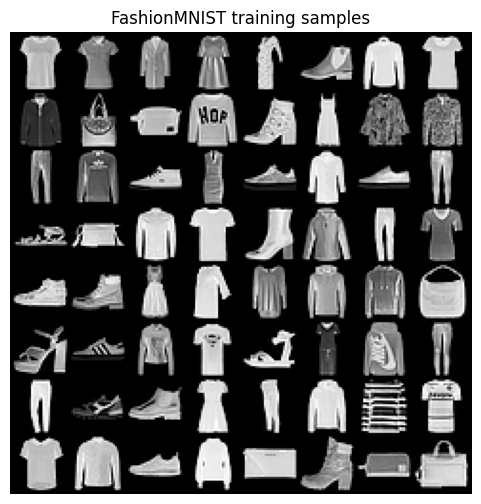
\includegraphics[width=0.58\linewidth]{figures/writeup/problem_5_c_i_dataset.png}
\end{center}

\subsection*{Problem 5.C.ii: Training Curves}
The VP-SDE model was trained for 50 epochs with $[\beta_{\min},\beta_{\max}]=[0.01,10]$, batch size $64$, and learning rate $10^{-4}$.  I did not use early stopping; the model was checkpointed after each epoch.  The loss drops quickly in the first few epochs and then decreases more gradually, indicating that most coarse denoising structure is learned early while later epochs refine the score estimates.

\begin{center}
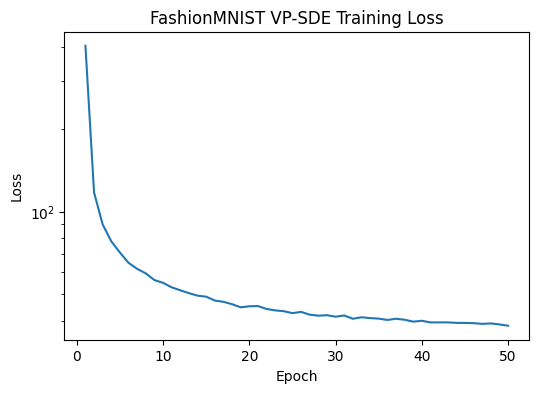
\includegraphics[width=0.68\linewidth]{figures/writeup/problem_5_c_ii_loss.png}
\end{center}

\subsection*{Problem 5.C.iii: EM Samples}
\begin{center}
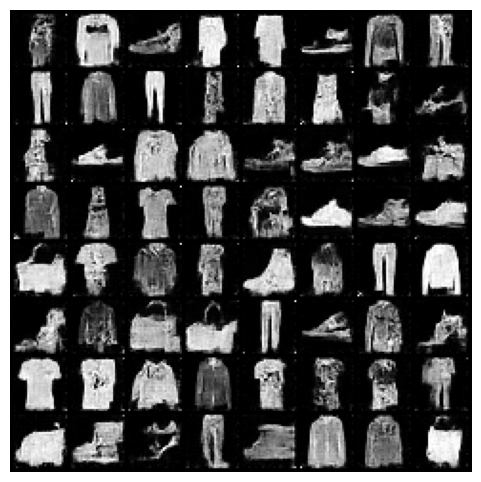
\includegraphics[width=0.58\linewidth]{figures/writeup/problem_5_c_iii_em.png}
\end{center}

\subsection*{Problem 5.C.iv: PC Samples}
The first grid uses one corrector step per predictor step.  The second grid uses five corrector steps.

\begin{center}
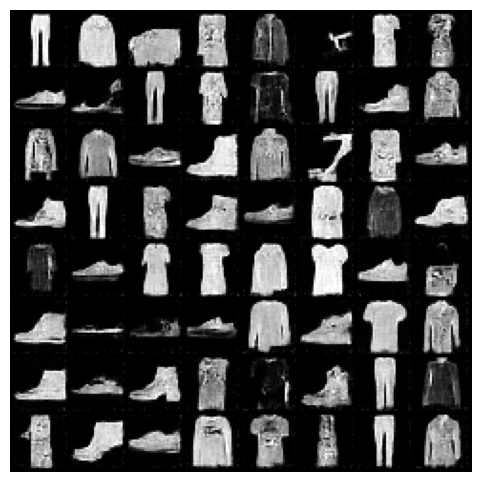
\includegraphics[width=0.48\linewidth]{figures/writeup/problem_5_c_iv_pc1.png}
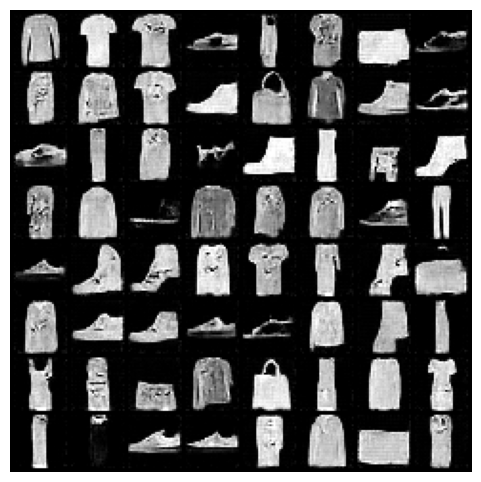
\includegraphics[width=0.48\linewidth]{figures/writeup/problem_5_c_iv_pc5.png}
\end{center}

\subsection*{Problem 5.C.v: Qualitative Discussion}
All samplers produce recognizable FashionMNIST-like objects, especially shoes, shirts, trousers, bags, and ankle boots.  The EM samples are already coherent but have more speckled texture and occasional distorted shapes.  Adding corrector steps makes the samples slightly sharper and more class-like, although using five corrector steps still leaves some grainy artifacts and does not perfectly recover fine clothing details.  Relative to the training set, the model captures the broad silhouettes well but struggles with crisp edges, printed patterns, and some of the less common class-specific details.

\subsection*{Problem 5.D: Diffusion Models for Inverse Problems}
The notebook conditions the reverse process on the observed pixels by repeatedly blending the current reverse-SDE sample with a noisy version of the corrupted measurement at the same diffusion time.  The diagonal inpainting matrix $A$ preserves observed pixels and leaves missing pixels to be filled by the score model.  The conditioning weight is scheduled with time so that the reverse process remains close to the measurement while still allowing the score model to generate plausible missing structure.

\begin{center}
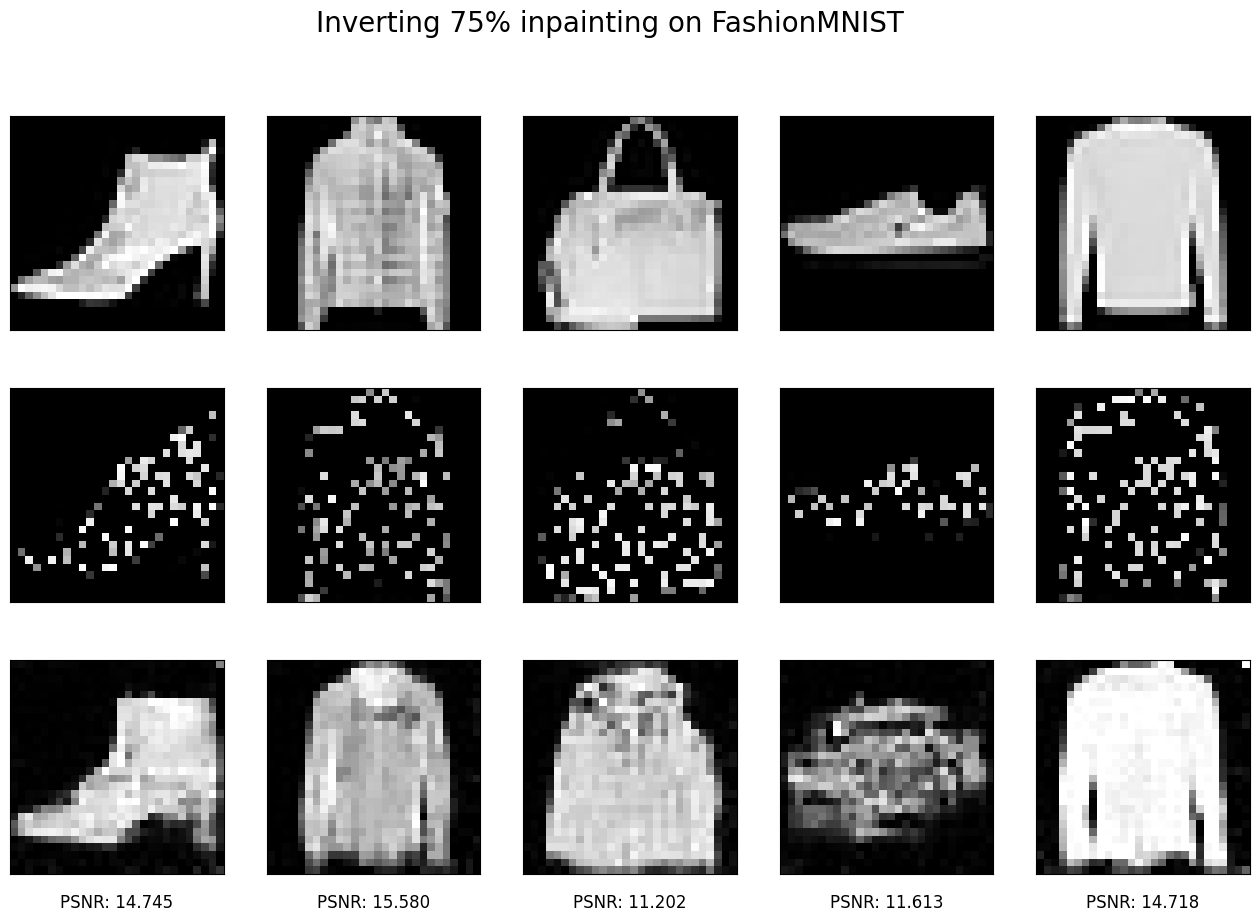
\includegraphics[width=0.9\linewidth]{figures/writeup/problem_5_d_inpainting.png}
\end{center}

With 75\% of pixels removed, the reconstructions preserve broad class identity and recover plausible silhouettes, but they are visibly blurred and noisy.  The reported PSNR values, approximately 11--16 dB, reflect that the inverse problem is highly underdetermined at this corruption level.  The conditioning step is helpful because it anchors observed pixels during the reverse process, while the score model fills the missing region with samples that stay near the FashionMNIST prior.

\subsection*{Problem 6.A: Rectified Flow Training}
For rectified flow, I trained a velocity network $v_\theta(x_t,t)$ on FashionMNIST using the interpolation
\[
x_t=(1-t)x_0+tx_1,\qquad x_0\sim\N(0,I),\quad x_1\sim p_{\mathrm{data}},
\]
and the mean-squared velocity objective
\[
\mathcal L_{\mathrm{RF}}(\theta)
=\E_{t,x_0,x_1}\left[\left\|v_\theta(x_t,t)-(x_1-x_0)\right\|^2\right].
\]
The VP baseline was trained for 48 epochs before early stopping, with best validation loss $0.0752$.  The first rectified-flow model was trained for 50 epochs, decreasing from loss $0.4080$ to best loss $0.2239$.  Reflow was then trained for 20 epochs after generating $50{,}000$ paired samples using 100 Euler steps; its loss decreased from $0.1665$ to $0.0133$.

\subsection*{Problem 6.B: KID Comparison}
The table reports Kernel Inception Distance using $1000$ generated FashionMNIST samples for each method and step count.  The reported standard deviation is zero because the evaluation used one $1000$-sample subset.

\begin{center}
\begin{tabular}{lrr}
\toprule
Method & Steps & KID \\
\midrule
Flow Matching & 1 & 0.384621 \\
Flow Matching & 5 & 0.019559 \\
Flow Matching & 10 & 0.008438 \\
Flow Matching & 50 & 0.006261 \\
Flow Matching & 100 & 0.006430 \\
Flow Matching & 200 & 0.006565 \\
Flow Matching & 1000 & 0.006786 \\
DDIM & 1 & 0.203306 \\
DDIM & 5 & 0.128408 \\
DDIM & 10 & 0.122928 \\
DDIM & 50 & 0.109964 \\
DDIM & 100 & 0.108363 \\
DDIM & 200 & 0.108069 \\
DDIM & 1000 & 0.108044 \\
DDPM EM & 1 & 0.502270 \\
DDPM EM & 5 & 0.389101 \\
DDPM EM & 10 & 0.281120 \\
DDPM EM & 50 & 0.126093 \\
DDPM EM & 100 & 0.089070 \\
DDPM EM & 200 & 0.072910 \\
DDPM EM & 1000 & 0.064490 \\
\bottomrule
\end{tabular}
\end{center}

Rectified flow improves very quickly as the Euler step count increases: one step is poor, but five steps already beats both diffusion baselines in this run, and the best KID occurs around 50 steps.  DDIM improves only modestly with more steps and plateaus near $0.108$, while DDPM Euler-Maruyama improves more steadily but remains worse than the multi-step rectified-flow sampler at 1000 steps.  This behavior matches the geometry of the methods: rectified flow learns a direct transport velocity, so coarse Euler integration can be accurate if trajectories are nearly straight; DDPM follows a stochastic reverse process and therefore pays a larger discretization cost at small step counts.

\subsection*{Problem 6.C: Reflow}
Reflow forms new training pairs by sampling $x_0\sim\N(0,I)$, transporting $x_0$ through the learned rectified-flow ODE to obtain $\hat x_1$, and retraining on the deterministic pairs $(x_0,\hat x_1)$.  In the run above, the reflow loss fell to $0.0133$, much lower than the first rectified-flow loss, indicating that the second model is fitting substantially straighter and more consistent trajectories.  Qualitatively, this should improve the one-step sampler because after reflow the desired displacement is closer to a single constant velocity from the source point to its transported endpoint.

\subsection*{Problem 6.D: Side-by-Side Comparison}
The Colab notebook generates the requested $4\times 8$ comparison grid at \texttt{runs/comparison\_grid.png}, with rows corresponding to DDPM EM with 1000 steps, rectified flow with 100 steps, rectified flow with 1 step, and reflow with 1 step.  The expected qualitative pattern is consistent with the KID table: many-step rectified flow should be the cleanest among the tested methods, one-step rectified flow should be visibly under-integrated, and one-step reflow should recover much more coherent FashionMNIST shapes than the original one-step flow.

\subsection*{Problem 7.1: Unconditional Image Generation}
The unconditional run used:
\begin{verbatim}
MODEL_FLAGS="--attention_resolutions 32,16,8 --class_cond False
--diffusion_steps 1000 --image_size 256 --learn_sigma True
--noise_schedule linear --num_channels 256 --num_head_channels 64
--num_res_blocks 2 --resblock_updown True --use_fp16 True
--use_scale_shift_norm True"
SAMPLE_FLAGS="--batch_size 8 --num_samples 8 --timestep_respacing 250"
python scripts/image_sample.py $MODEL_FLAGS \
--model_path models/256x256_diffusion_uncond.pt $SAMPLE_FLAGS
\end{verbatim}

\begin{center}
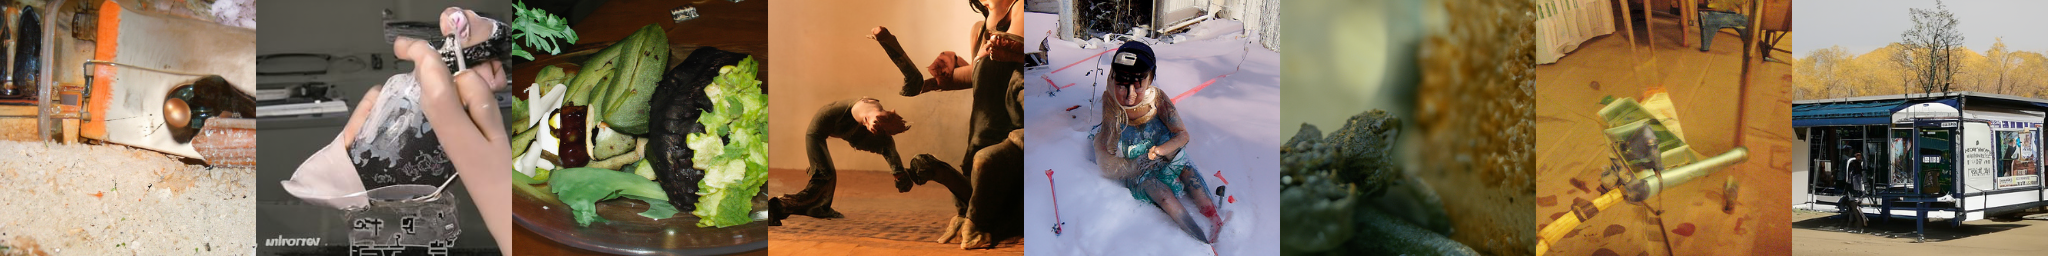
\includegraphics[width=\linewidth]{figures/writeup/problem_7_1_unconditional.png}
\end{center}

The generated images are diverse and contain recognizable ImageNet-like scenes and objects, including indoor objects, food-like textures, people, and outdoor structures.  Some samples are realistic at first glance, while others show typical diffusion artifacts such as warped object boundaries, inconsistent local geometry, and unusual object blends.

\subsection*{Problem 7.2: Progressive Generation}
The progressive visualization was generated by running the unconditional sampler with the same model flags as Problem 7.1 and saving evenly spaced states from the progressive sampling loop, starting with the initial Gaussian noise and ending with the final sample.

\begin{center}
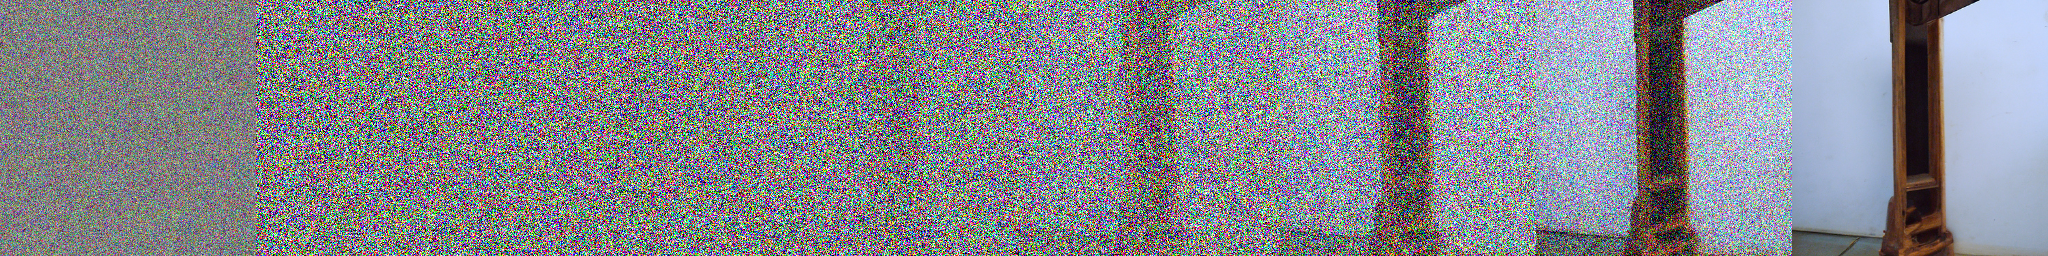
\includegraphics[width=\linewidth]{figures/writeup/problem_7_2_progressive.png}
\end{center}

The early columns are dominated by high-frequency noise, then coarse color fields and large shapes emerge, and the final columns contain the recognizable image structure.  This illustrates the coarse-to-fine nature of reverse diffusion: global layout stabilizes before small details become clean.

\subsection*{Problem 7.3: Noise Interpolation}
Two distant Gaussian noise vectors were chosen from a fixed random seed, and eight linearly interpolated noise vectors were sampled:
\[
z_i=\left(1-\frac{i}{7}\right)z_0+\frac{i}{7}z_7,\qquad i=0,\ldots,7.
\]

\begin{center}
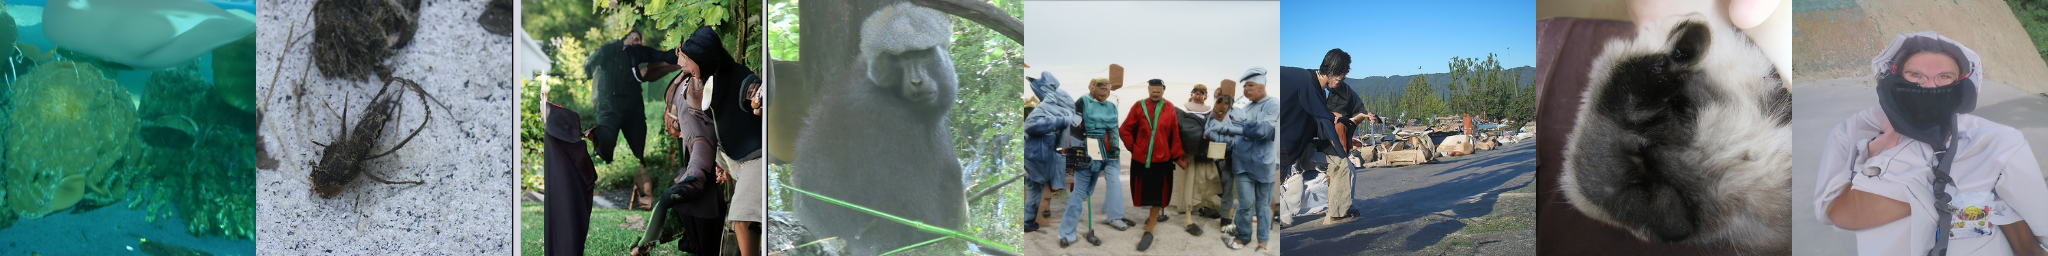
\includegraphics[width=\linewidth]{figures/writeup/problem_7_3_interpolation.png}
\end{center}

The endpoints produce visually distinct samples, and the intermediate samples move through different semantic regions of the model's latent/noise space.  The interpolation is not a simple pixel-space morph; instead, semantic content can change abruptly because the denoising process maps nearby noise vectors through a highly nonlinear generative trajectory.

\subsection*{Problem 7.4: Conditional Image Generation}
The conditional run used the same unconditional diffusion model together with the noisy ImageNet classifier:
\begin{verbatim}
CLASSIFIER_FLAGS="--classifier_attention_resolutions 32,16,8
--classifier_depth 2 --classifier_width 128 --classifier_pool attention
--classifier_resblock_updown True --classifier_use_fp16 True
--classifier_use_scale_shift_norm True --image_size 256"
python scripts/classifier_sample.py $MODEL_FLAGS $CLASSIFIER_FLAGS \
--classifier_scale 10.0 --classifier_path models/256x256_classifier.pt \
--model_path models/256x256_diffusion_uncond.pt $SAMPLE_FLAGS
\end{verbatim}

\begin{center}
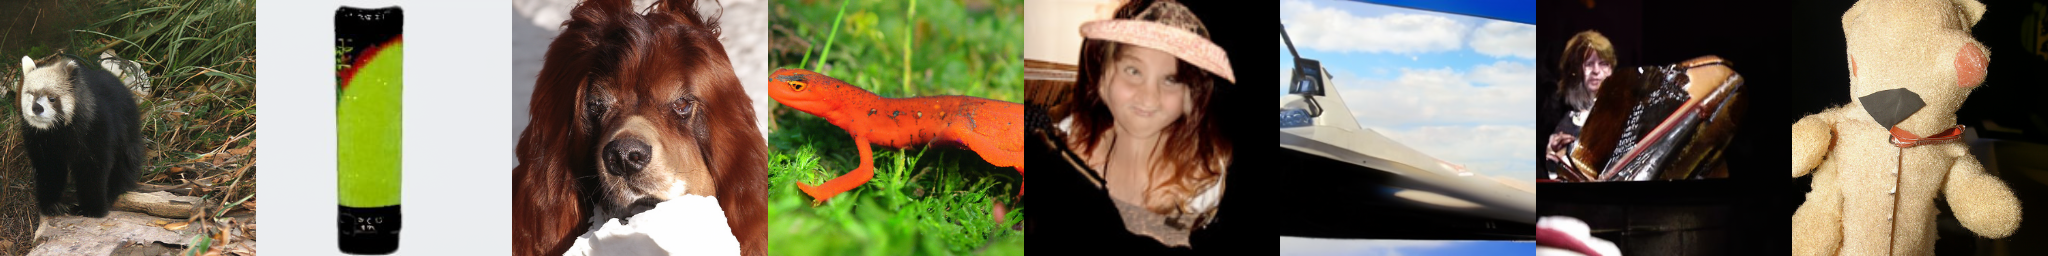
\includegraphics[width=\linewidth]{figures/writeup/problem_7_4_conditional.png}
\end{center}

Classifier guidance makes the samples more object-centric and often sharper than the purely unconditional run.  The grid contains several clear object-like samples, although some images still show distorted backgrounds or implausible local details, especially around fine structures.

\subsection*{Problem 7.5: Classifier Scale Sweep}
The sweep used classifier scales
\[
0,\ 0.25,\ 0.5,\ 1,\ 2,\ 4,\ 8,\ 12.
\]

\begin{center}
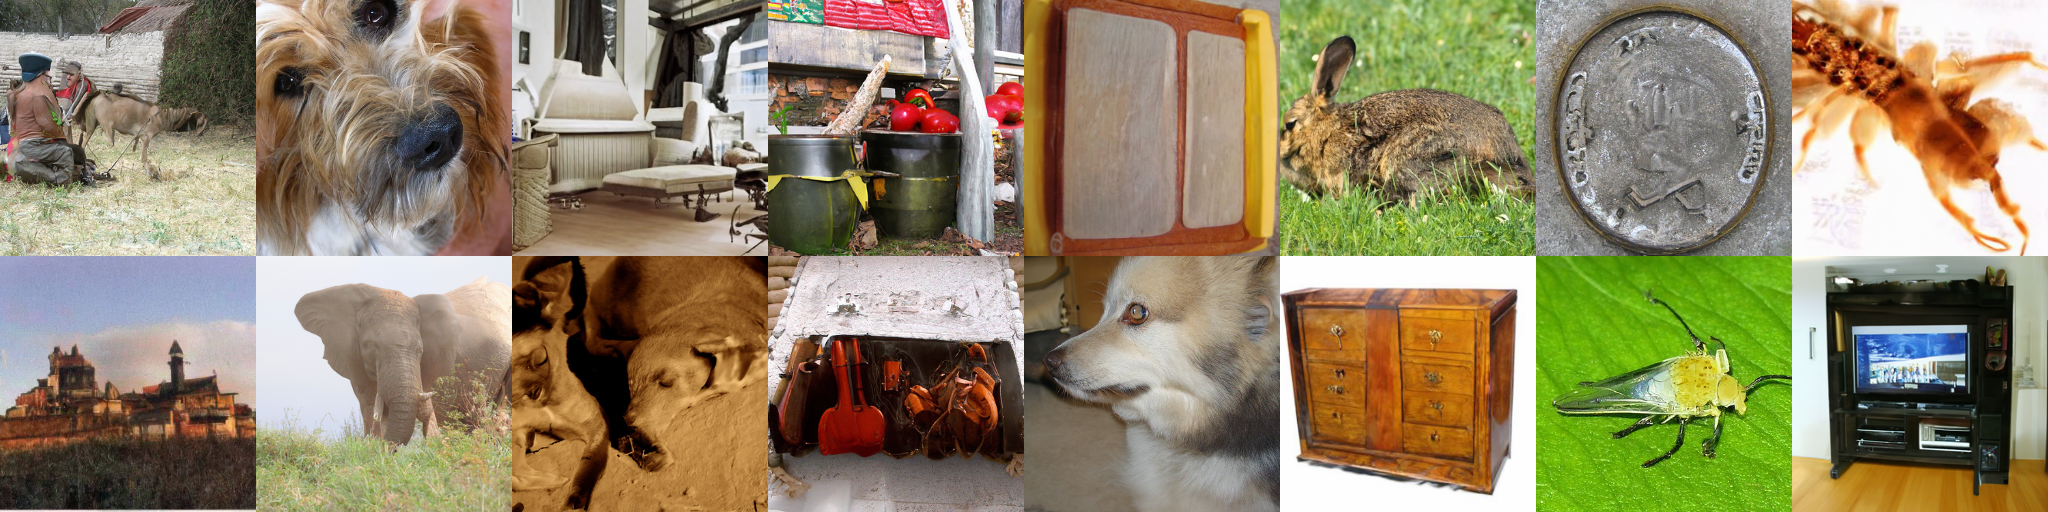
\includegraphics[width=\linewidth]{figures/writeup/problem_7_5_scale_sweep.png}
\end{center}

At low classifier scale, samples are more diverse but less strongly class-directed.  As classifier scale increases, objects become more salient and high-contrast, but the model also becomes more prone to oversaturated textures, reduced diversity, and strange local artifacts.  This matches the usual classifier-guidance tradeoff: stronger guidance improves class confidence but can sacrifice naturalness and diversity.

\end{document}
